%!tex root = ../report.tex

\section{Antipatterns}
\textit{\large If one does not know how to solve a problem, it may nevertheless be useful to know about likely blind alleys.}
\begin{flushright}
	--- Andrew Koenig
\end{flushright}

Antipatterns are typical mistakes in software development. The most common reasons for such mistakes can be found in the seven deadly sins in software practice:\newline

\begin{tabular}{ll}
	\textbf{Apathy} & Not caring about a problem, unwillingness to attempt a solution \\ 
	\textbf{Haste} & Solutions based on hasty decisions \\ 
	\textbf{Narrow-mindedness} & The refusal to use solutions that are widely known \\ 
	\textbf{Sloth} & Making poor decisions based on "easy" answers \\ 
	\textbf{Avarice (excessive complexity)} & No use of abstractions, excessive modeling of details \\ 
	\textbf{Ignorance} & Failure to seek understanding \\ 
	\textbf{Pride} & Not invented here: Not willing to adopt anything from the outside
\end{tabular}
\vspace{0.5cm}
\newline
There are three roles in software development: developer, architect, manager. Antipatterns can also be split up into those three areas:\newline

\textbf{Developer Antipatterns:}
Focus on the viewpoint of the \textit{software developer}.\newline
\texttt{Issues}: software refactoring, modification of source code to
improve the software structure with respect to long-term
maintainability.\newline
\textbf{Architecture Antipatterns}
Focus on the viewpoint of the \textit{software architect}.\newline
\texttt{Issues}: partitioning of subsystems and components, platform
independent definition of interfaces, and connectivity of
components.\newline
\textbf{Management Antipatterns}
Focus on the viewpoint of the \textit{software project manager}.\newline
\texttt{Issues}: software project organization, software project
management, software process model, human communication,
rationale management and resolution of issues.\newline

\subsubsection*{Definition of Antipattern}
An Antipattern consists of a problem and two solutions.
The \textit{problematic} solution describes a commonly occurring solution that generates overwhelming negative consequences.
The \textit{refactored} solution describes how the problematic solution can be reengineered to avoid these negative consequences and lead to benefits again. 
The Refactored Solution leads to \textit{Follow-On Problems} which again can be elaborated in terms of Context and Forces and may lead to the applicability of other patterns.\newline

Patterns can evolve into antipatterns when changes occur.
Such changes can be for example in requirements, project parameters or the methodology.
In those cases, the solution proposed by the pattern becomes a problematic solution.
\newpage

\begin{figure}[h]
	\centering
	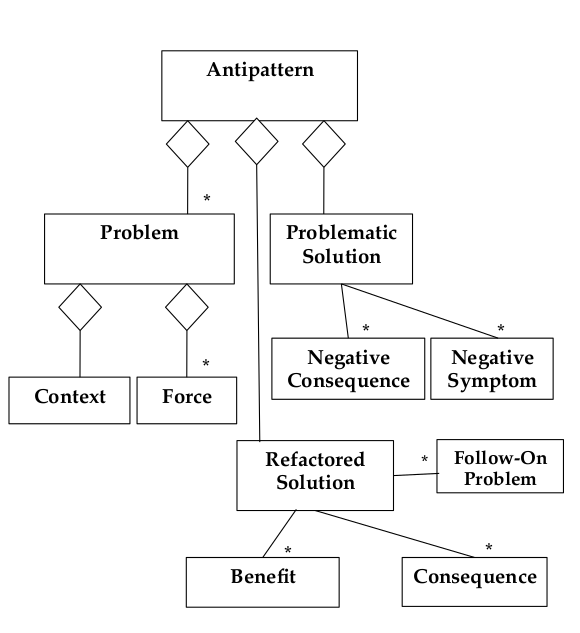
\includegraphics[width=0.7\linewidth]{images/antipattern}
	\caption{Definition of Antipattern}
\end{figure}

\newpage

\subsection{Functional Decomposition Antipattern}
Functional decomposition describes the decomposition of a system in terms of functions instead of use cases and/or objects (object-oriented decomposition) so that functions are hidden somewhere in the system where nobody might expect them.

\textit{Recommended approach:} First decompose the system in use cases, then in objects.

\begin{description}
  \item[General Form] Everything is a function, lots of files named misc, util,aux,...
  \item[Symptoms and Consequences] \hfill
  \begin{itemize}
    \item Maintainer must understand the whole system to make changes
     \item Code is hard to understand
     \item Code is complex, high coupling between code sections in different files
     \item User interface is often awkward and non-intuitive
  \end{itemize}
  \item[Typical Causes] Wrong trained personal (programmers, designers)
\end{description}
\newpage

\subsection{Golden Hammer Antipattern}
Everything is solved with a specific tool.
\begin{description}
	\item \textbf{General Form}
	\begin{itemize}
		\item Developer has high level of competence in a particular solution
	    \item Every new development effort is solved with this solution
	    \item Developer is unwilling to learn and apply new approach
	\end{itemize}
	\item \textbf{Symptoms and Consequences}
	\begin{itemize}
	  	\item Identical tools used for many diverse products
	  	\item System architecture depends on a particular application suite and a
  	specific vendor tool set
	\end{itemize}
	\item \textbf{Typical Causes}
	\begin{itemize}
	  	\item Large investment in product for specific technologies maybe with exclusive features.
	  	\item Reliance on proprietary product features that are not available from
	  	other vendors or products
	\end{itemize}
	\item[Known Exceptions] Product is part of a vendor suite that provides for all needs
\end{description}
\newpage

\subsection{Lava Flow}
Also known as dead code.
\begin{description}
  \item \textbf{General Form} Lava like flows of previous development hardened into a basalt like mass of code, difficult to remove once solidified.
  \item \textbf{Symptoms and Consequences}
  \begin{itemize}
    \item Unused or commented-out code
    \item Undocumented complex, important-looking code
    \item Functions or classes that do not relate to the system architecture
    \item Evolving architecture
  \end{itemize}
  \item \textbf{Typical Causes}
  \begin{itemize}
    \item Research and development code placed into production
    \item Implementation of several trial approaches
    \item High programmer turnover rate
    \item Fear of breaking something and not knowing how to fix it
    \item Unclear, repeatedly changing project goals
    \item Architectural scars
  \end{itemize}
  \item \textbf{Exceptions} Small-scale, rapidly developed throwaway prototypes
\end{description}
\newpage

\subsection{Blob Antipattern}
Also known as god class
\begin{description}
  \item \textbf{General Form} Majority of responsibilities are in one complex controller and are associated with simple data classes.
  \item \textbf{Symptoms and Consequences}
  \begin{itemize}
    \item Huge class with many unrelated attributes and operations encapsulated
    \item The blob is usually to complex to reuse and testing
  \end{itemize}
  \item \textbf{Typical Causes}
  \begin{itemize}
    \item Lack of (object-oriented) architecture
    \item Too limited intervention in iterative projects
  \end{itemize}
  \item \textbf{Known Exceptions} Wrapping of legacy systems
\end{description}
\newpage

\subsection{Spaghetti Code Antipattern}
Ad hoc structure which makes it hard to extend or optimize the code.
\begin{description}
  \item[General Form] Software with very little structure where object methods are invoked in a single, multistage process flow
  \item[Symptoms and Consequences] \hfill
  \begin{itemize}
    \item Methods are process oriented, objects are named as processes
    \item Execution flow is dictated by the class implementation of objects instead by the users of that class
    \item No inheritance, no polymorphism
    \item Source code difficult to reuse
    \item Point of diminishing returns: the software maintenance effort is higher than a complete re-engineering effort
  \end{itemize}
  \item[Typical Causes] \hfill
  \begin{itemize}
    \item No design prior to implementation
    \item Inexperience with object-oriented design
  \end{itemize}
\end{description}
\newpage

\subsection{Vendor Lock-In Antipattern}
Dependence on a proprietary architecture or tool set, making it hard to switch to
another vendor.
\begin{description}
  \item[General Form] A software project adopts product technology and becomes completely dependent of the vendor's implementation
  \item[Symptoms and Causes] \hfill
  \begin{itemize}
    \item Maintenance cycle driven by the product update cycle
    \item Promised product features are delayed or never delivered, subsequently, causing failure to deliver application updates
    \item Application programming requires in-depth product knowledge
  \end{itemize}
  \item[Typical Causes] \hfill
  \begin{itemize}
    \item Product is selected because of marketing instead of technical inspection
    \item Product varies from published open system standards because there is no effective conformance process for the standard.
  \end{itemize}
  \item[Known Exceptions] Single vendors code is the majority of the code needed for an application
\end{description}
\newpage

\subsection{Analysis Paralysis Antipattern}
Excessive time is spend in requirements analysis.
\begin{description}
  \item[General Form] \hfill
  \begin{itemize}
    \item Goal to achieve perfection and completeness of the analysis phase
    \item Very detailed models
  \end{itemize}
  \item[Symptoms and Consequences] \hfill
  \begin{itemize}
    \item Analysis cost exceeds expectations without a predictable end point
    \item Analysis documents no longer make sense to the domain experts
  \end{itemize}
  \item[Typical Causes] \hfill
  \begin{itemize}
    \item Management assumes waterfall progression of phases
    \item Analysis Goals are not well defined
  \end{itemize}
\end{description}
\newpage

\section{Code Smells and Refactoring}
\subsection{Code Smells}
Code smells are symptoms in the source code of a program that possibly indicate bigger problems. It is a heuristic indication, when to refactor and what specific technique to use.
\begin{description}[]
  \item \textbf{Method too long:} Extract method
  \item \textbf{Duplicated code:} Extract/pull up method, extract class
  \item \textbf{Class to large:} Extract superclass
  \item \textbf{Parameter list too long:} Replace parameter with explicit method, introduce parameter object
  \item \textbf{Feature envy (class uses methods of another class excessively):} Move class
  \item \textbf{Lazy class (no interesting behavior):} Turn class into attribute 
  \item \textbf{Speculative generality (exessive use on inheritance):} Collapse inheritance tree
  \item \textbf{Refused bequest (subclass reusing behavior of superclass, but interface not supported)}: Replace inheritance with delegation
\end{description}
\newpage

\subsection{Refactoring}
Refactoring can be partioned into six sections:

\begin{figure}[h]
	\centering
	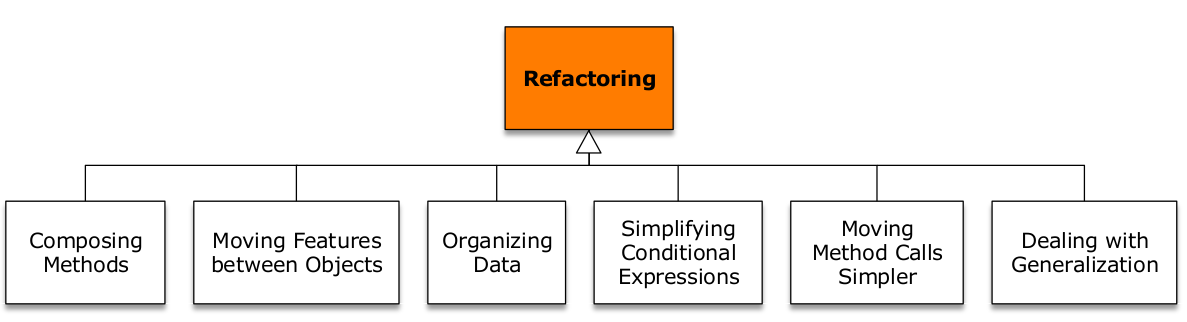
\includegraphics[width=\linewidth]{images/refactoring_taxonomy}
	\caption{Source Code Refactoring Taxonomy}
\end{figure}

The following lists a common refactoring technique for each of those sections.


\subsubsection*{Replace Inheritance with Delegation (\textit{Dealing with Generalization})}
In this case a subclass is only using parts of the superclass interface or does not want to inherit data.
This results in source code that says one thing when you intention is something else, which leads to confusion.

Here, the inheritance should be replaced with delegation.
This makes clear that only parts of the delegated class are used.\newline 

\textbf{Steps:}
\begin{enumerate}
	\item Create a field in the subclass that refers to an instance of the superclass
	\item In the subclass, call public methods of the superclass via this
	field
	\item Break the inheritance relationship by removing the extends declaration from the subclass definition
	\item Create delegating methods in the subclass for those
	superclass methods that you want to use in the subclass
\end{enumerate}

\subsubsection*{Extract Method (\textit{Composing Methods})}
This refactoring shortens methods by extracting methods.
For this, related parts of the method's body are extracted and moved to a separate method.

\subsubsection*{Extract Class (\textit{Moving Features between Objects})}
If a class contains an implicit abstraction that is not explicitly modeled (e.g. class \texttt{Person} with \texttt{officeAreaCode, officeNumber, privateAreaCode, privateNumber, ...}), the attributes can be summarized in a separate class (e.g. \texttt{TelephoneNumber}) and then used in the original class.

\subsubsection*{Replace Data Value with Object (\textit{Organizing Data})}
When a simple attribute of a class (e.g. class \texttt{Order} attribute \texttt{String customer}) gets more versatile (e.g. more information or an operation is needed), the value can be replaced by a object of a newly introduced class.

\subsubsection*{Replace Conditional with Polymorphism (\textit{Simplifying Conditional Expressions})}
A simple if-then-else may mutate to a switch-case statement over time.
As the possible cases grow, the code may become confusing and difficult to maintain.
In this case, polymorphism may be introduced.
For that, the object on which the decision is made is turned into an abstract class and subtypes encapsulating the different cases are introduced
(e.g. class \texttt{Bird}, attribute \texttt{size} can be made abstract and the subclasses \texttt{SmallBird}, \texttt{MiddleBird} and \texttt{LargeBird} may be introduced, compare \textit{Command Pattern}).

\subsubsection*{Replace Error Codes with Exceptions (\textit{Making Method Calls Simpler})}
When error codes are used (e.g. negative values) as return values of methods, developers using these methods often struggle with resolving these errors as the codes have to be looked up to get their meaning.
Instead exceptions can be used to transfer information on the error to the caller of a method.
This moves the responsibility to resolve the error to the caller.

\newpage
